\documentclass[aps,pre,twocolumn,letterpaper,floatfix,showpacs]{revtex4}
\usepackage{graphicx} 
\usepackage{amsmath,amssymb,amsfonts} 
\usepackage{mathtools}
\usepackage{pdfpages}
\usepackage{afterpage}
\usepackage[hidelinks]{hyperref} 
\usepackage{epstopdf}
\usepackage{siunitx}
\usepackage{color}
\definecolor{Blue}{rgb}{0.1,0.1,1.0} 
\definecolor{Magenta}{rgb}{1.0,0.1,0.5} 
\definecolor{LRed}{rgb}{0.8,0.0,0.0} 

 \newcommand{\todo}[1]{ {\color{Magenta} TODO: \color{Blue} \textbf{#1} }}


\begin{document}
\title{Structural replication of nanoporous media using procedural noise}
%\author{A. Hafreager, N. Groeneboom, A. Malthe-S\oe renssen$^1$}
\email{anders.hafreager@fys.uio.no}
\author{Anders Hafreager $^{1}$} 
\author{Nicolaas Groeneboom $^{1}$} 
\author{Anders Malthe-S\o renssen $^1$}
\affiliation{$^1$Department of Physics - University of Oslo\\Sem S{\ae}lands vei 24, NO-0316, Oslo, Norway }
\date{\today} 

%%%%%%%%%%%%%%%%%%%%%%%%%%%%%%%%%%%%%%%%%%%%%%%%%%%%%%%%%%%%%%
%%%%%%%%%%%%%%%%%%%%%%%%%%%%%%%%%%%%%%%%%%%%%%%%%%%%%%%%%%%%%%
\begin{abstract} 
In this paper, we aim to develop a method for producing statistically correct porous media using noise functions. In short, the proposed model is a binary function that returns either true if the input point is inside pore space, or false if within a wall. By using procedural noise, we are not restricted to generating media within a limited box, as the noise functions is continuous on all scales. It is therefore possible to generate geometries at arbitrary scales. In addition, this method is extremely fast and has low memory footprints, requiring very little computational power. After presenting such a model, we choose a method to measure the structural properties of nanoporous media that are created either through regular methods (e.g. molecular dynamics) or with our method. The radial distribution function $g(r)$ is chosen as a measure of the structural properties to compare the simulated geometry to our model. Using this measure, we define a full likelihood framework for estimating model parameters given any data set, and continue by validating our own framework by analysing procedural noise data sets with known input parameters. Finally, we generate a nanoporous media with an expand-and-quench technique using molecular dynamics and show that our model correctly reproduces several of the internal properties of the data set, including $g(r)$, porosity and surface area.  \todo{Abstract boer tenkes noe gjennom: faa frem hovedpoenger.}   

\end{abstract} 
 
\maketitle
 
% %%%%%%%%%%%%%%%%%%%%%%%%%%%%%%%%%%%%%%%%%%%%%%%%%%%%%%%%%%%%%
%% %%%%%%%%%%%%%%%%%%%%%%%%%%%%%%%%%%%%%%%%%%%%%%%%%%%%%%%%%%%%
\section{Introduction}

%During recent years, increase in computational power has allowed for a vast improvement  
\todo{Skriv en fin intro! Ogsaa om nanoporous media}
Properties of structural patterns that regularly occur in nature are often investigated either through direct observations or through simulations of theoretical models. Model simulations typically require a large computational framework to accurately reproduce the observed effects, while experimental data can be both expensive and hard to obtain, in addition to being riddled with artefacts and instrumental errors.   

Procedural generation of physical structures have several advantages over conventional simulations. For example, when producing simulations of nanoporous silica, we are required to calculate and propagate the physical properties of each particle for every time-step throughout the simulation, using a computational framework such as LAMMPS \cite{plimpton1995fast}. This is both time-consuming, and the computational cost can sometimes be be quite large. In addition, the simulation is constrained to a box, so particles are not allowed to move outside the defined boundaries. On the other hand, using procedural noise to carve out nanoporous media is both extremely fast and computationally cost-efficient, in addition to being continuous on all scales. This means that it is possible to simulate 
\todo{Nevn finite size effects}
%In addition, by creating a model that yields properties that are statistically consistent with observations, we are ar

In this paper, we aim to investigate whether procedural methods are suitable for producing statistically correct 3D physical structures, focusing on nanoporous media. In a sense, we are combining well-known methods from computer games and real-time graphics-oriented software with experimental observations and simulations. Procedural methods for automated generation of computer game content have been around since the early 1980's, and in those early days algorithms were less advanced, often yielding plain, simple geometrical structures. Nowadays, almost every single computer game produced will contain some level of automated generated content, from textures to level design to landscapes and gameplay. 

We do not claim that procedural noise methods completely reproduces all structural properties of nanoporous silica, but show that our approach can be used to efficiently create materials that are structurally similar to simulations. Naturally, this all depends on the statistics used for comparing the two models, which in this case is based on the radial distribution function $g(r)$ (RDF). 
\todo{Nevne at kjemi naturligvis ikke vil være riktig siden antall naboer per atom ikke er riktig. }
%\section{Method}
\section{Procedural content generation}
By procedural content generation, we generally mean a mathematical algorithm that uses limited input data to create complex, sometimes infinite repeating patterns. A firm example would be fractals, such as the Julaia/Mandelbrot [ref mandelbrot] set, where one tests whether the complex quadratic recurrence equation $z_{n+1} = z_n^2 +C$ for $z \in \mathbb C$ converges for each position in a 2D complex plane. With this seemingly simple equation, the level of complexity generated on the boundary between convergence and divergence is infinite, with self-similar patterns repeating themselves to arbitrary detail.
\begin{figure}
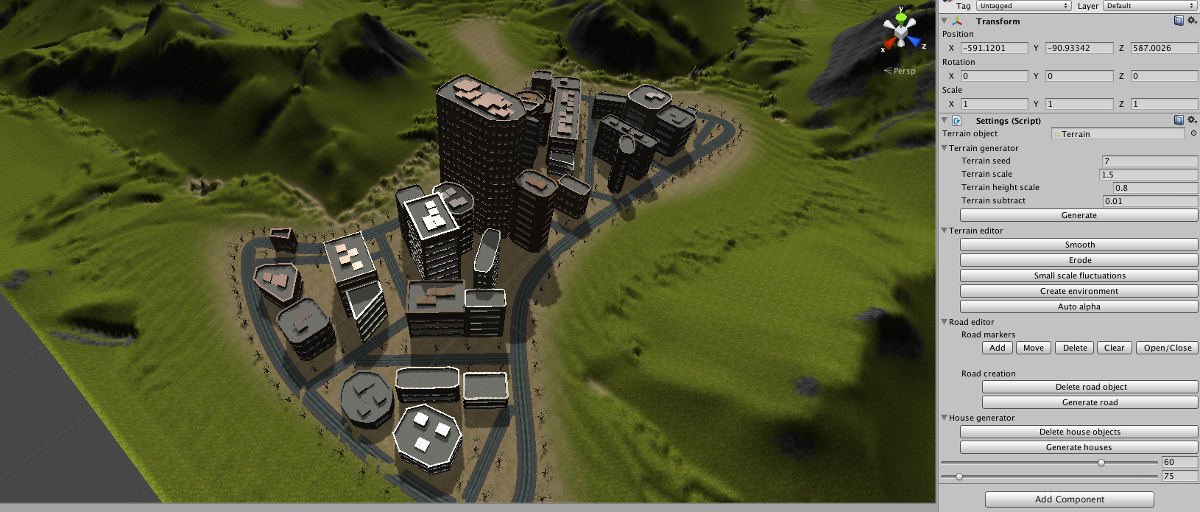
\includegraphics[width=.5\textwidth]{orphancity.png}
\caption{Example of city building using procedural methods: Landscape, city infrastructure, buildings and all textures are all automatically generated using procedural methods. Created by one of the authors. \todo{Denne er jo med bare for moro skyld, boer jo fjernes} }
\label{fig:orphancity}
\end{figure}

Another example, widely used in contemporary game content generation, is having prefabs (pre-fabricated 3D models such as doors, walls, tiles and roof segments) automatically being stitched together to create buildings. When designing a city, instead of creating each building manually, you only need specify the position, area and height of a structure. Then, by using an algorithm that combines these prefabs to render the building, it is possible to create cities of arbitrary size with a single command. Naturally, it is also possible to create procedural methods that design the layout and placement of these buildings. See figure \ref{fig:orphancity} for an example of such a city generator tool, developed by one of the authors of this paper. 

A much simpler example would be generating a 1 (or 2)-dimensional landscape by choosing random points on a grid and performing a spline interpolation between them to create the illusion of a smooth landscape. In fact, this is the very essence of procedural noise, which we are focusing on in this paper, and the first person to create such a fast algorithm for N-dimensional spline interpolation between pseudo-random points was Ken Perlin.   

\subsection{Perlin/Simplex noise}
\label{sec:perlin}

Procedural algorithmic methods for creating realistic-looking
fractal-like patterns have been around for more than 30 years. The most famous of these
algorithms is Perlin noise, first developed by Ken Perlin in 1983 for
use in the movie ``Tron''\cite{perlin1985image}. 

Perlin noise is a type of pseudo-random gradient noise that mimics a Gaussian field, but at low computational cost. An improved version of Perlin noise is called simplex noise, which has several advantages over standard Perlin noise in terms of scalability and speed \cite{perlin:2002}. Perlin noise was developed in response to the lack of detail 1980's contemporary graphics, where polygonal surfaces often were bland and left without any detail. In response to this problem, Perlin noise was developed in order to continuously perturb the light bouncing off flat surfaces, effectively yielding bump mapping and producing a much more realistic image. 

An overview of the current state of procedural noise functions can be
found in \cite{lagae:2010}. Perlin noise is a band limited repeatable pseudo-random function
from $\mathbb R^n \to \mathbb R$ that is computationally fast, and has
properties which make it suitable for creating patterns that mimic
nature. Perlin noise is an approximation to Gaussian filtered noise
implemented as a pseudo-random spline. The algorithm uses a predefined
grid of gradients pointing in a random direction, where for any point
within a grid, we interpolate the gradients from the four corners. The
algorithm is as follows:
\begin{itemize}
  \item[1.] For a point, obtain the four closest gradients in the grid.
   \item [2.] For each of the gradients, calculate the dot product
     between the gradient and a vector defined by the  the distance
     between the the point and the current grid corner. 
   \item [3.] Instead of linear interpolation $F(t) = t$, use a fade function to produce smoother interpolated values. Perlin noise typically uses the following fade function: $F(t) = t ^3 (t  (6 - 15) + 10)$.
    \item [4.] Obtain the final value by linearly interpolating between the x-axis and
      use this result to linearly interpolate the y-axis. 
\end{itemize} 
Simplex noise works in a similar manner, but works on on simplices instead of hypergrids, and so requires fewer computational steps, scales better in higher ($\ge 3$) dimensions and has fewer anisotropic properties. 

\subsection{Properties of Perlin/simplex noise}
\begin{figure}
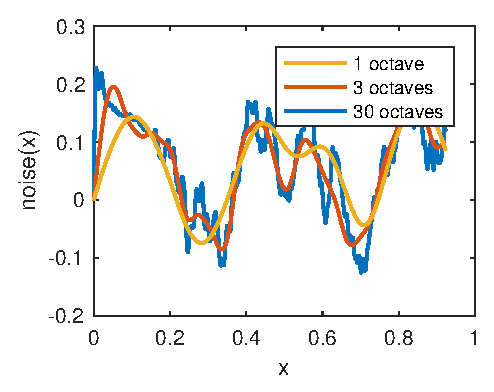
\includegraphics[width=.5\textwidth]{noise.eps}
\caption{Perlin noise (left) versus simplex noise (right). Note the
  straight x-y pattern in the single upper Perlin mode and the less
  anisotropic simplex mode. Lower part: combining octaves tend
  to remove these patterns.}
\label{fig:noise}
\end{figure}

\begin{figure}
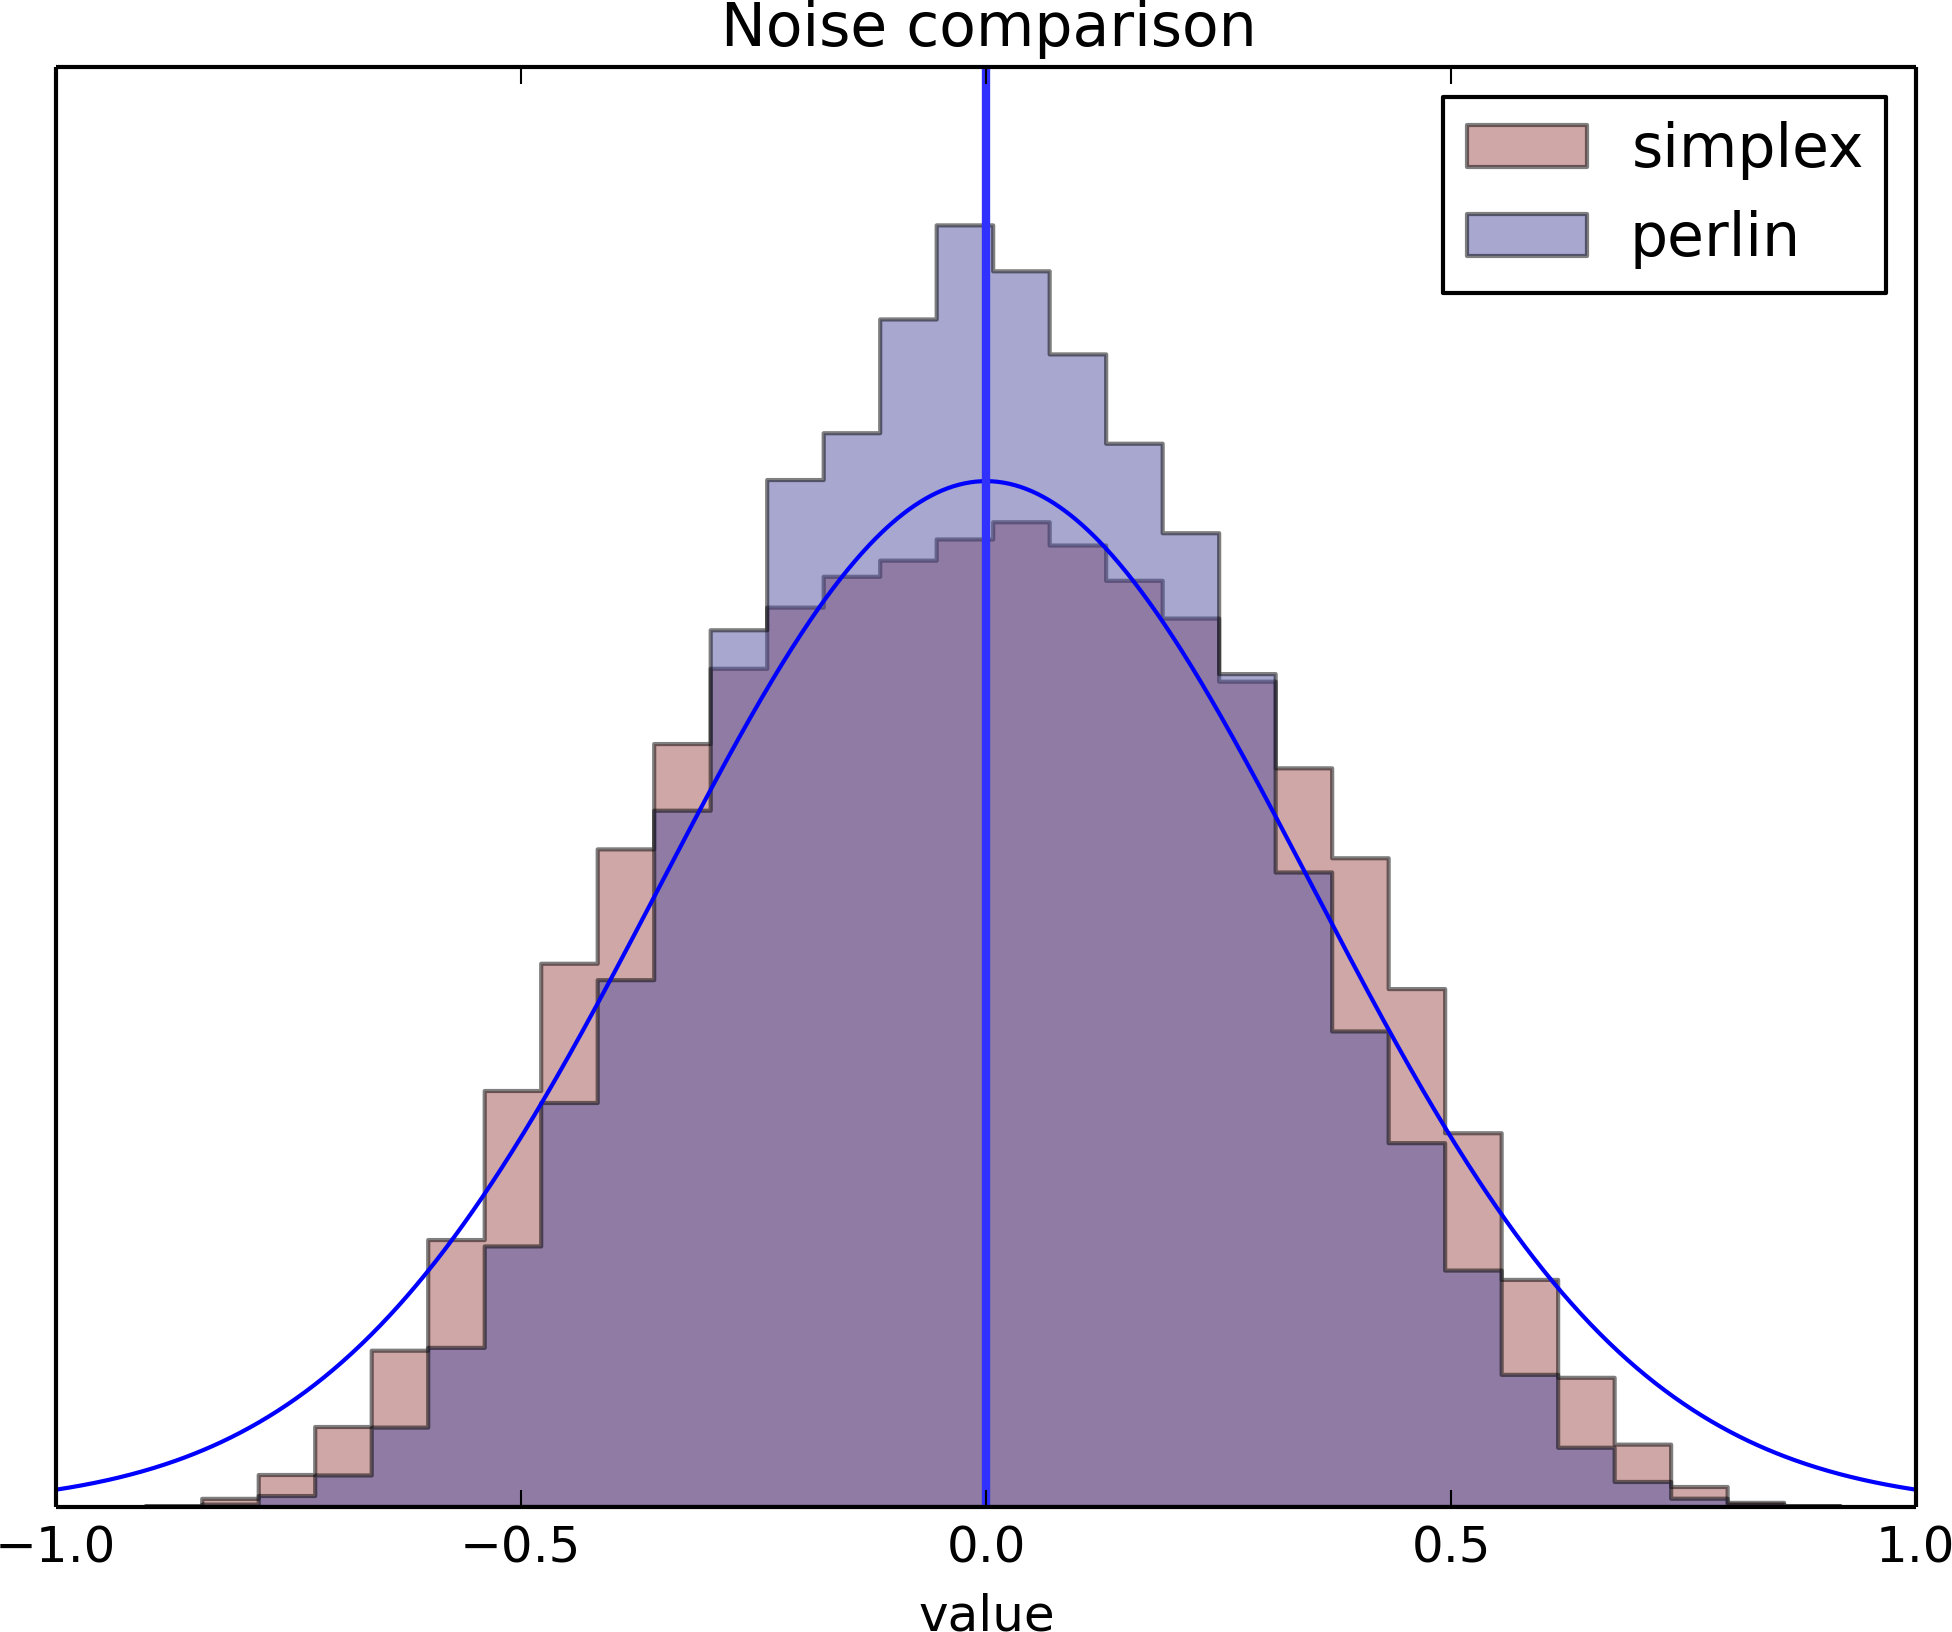
\includegraphics[width=.5\textwidth]{noise_comparison.png}
%\mbox{\epsfig{file=perlinstats.eps, width=\linewidth}}
\caption{Normalized distributions of Perlin noise and simplex noise compared with a
  Gaussian distribution. Note how both noise functions produce
  near-Gaussian, but slightly different distributions.}
\label{fig:properties}
\end{figure}
Standard Perlin noise is known for having several anisotropic features
\citep{lagae:2010}. Perlin noise also gives rise to a ``textile''
pattern in the $x$ and $y$-directions, which is evident from the upper
left part of figure \ref{fig:noise}, depicting 2D Perlin noise in
a single octave. The upper-right part shows the same node for simplex noise,
with less obvious patterns. However, when combining several octaves and adding a random shift to the coordinates,
as depicted in the two lower parts, these anisotropic patterns tend to cancel
out.  In addition, we have calculated the statistical distributions for Perlin and simplex noise
with $\sigma = 0.3$, and have plotted the results in figure \ref{fig:properties}.
Each procedural noise method has distributions that are close to normal, 
but with some asymmetrical properties. 



\subsection{Multiple octaves: creating patterns}
\label{sec:octaves}
The different octaves from procedural noise functions can be combined
to produce a wide range of nature-like patterns. A generic
N-dimensional procedural function $\Phi(\vec x): \mathbb R^N \to
\mathbb R$ could be expressed as
\begin{equation}
\label{eq:procedural}
 \Phi(\vec x) = \Theta \Big(\sum_k^\omega \kappa (k) P(  f_s (\vec x,k) )) \Big),
 \end{equation}
where $f_s(\vec x,k)$ describes the frequency scale modifier (e.g. $f_s(\vec x,k) =
k\vec x$), $\omega$ is the amount of octaves (modes), $\kappa(k)$ is the octave amplitude (e.g. $\kappa(k) = 1/k$)
and $\Theta(x)$ an overall modifier (e.g. $\Theta(x) = x$ or
$\Theta(x) = \frac{1}{x}$). In a sense, $\kappa(k)$ is similar to Fourier coefficients. 
In its simplest case, summing directly over the octaves with amplitude $1/k$ results in 
\begin{equation}
\label{eq:perlinlinear}
 \Phi(\vec x) = \sum_k^\omega \frac{1}{k} P( 2k\vec x).
\end{equation}
In 1 dimension, equation \ref{eq:perlinlinear} with 1, 3 and 30 octaves is depicted in figure \ref{fig:1dperlin}, while the 2D procedural noise pattern depicted in the lower
part of figure \ref{fig:noise}. Finally, since simplex noise both scales better with higher dimensions and produces less asymmetric effects, we choose to use this noise method over regular Perlin noise in our method.  

\begin{figure}
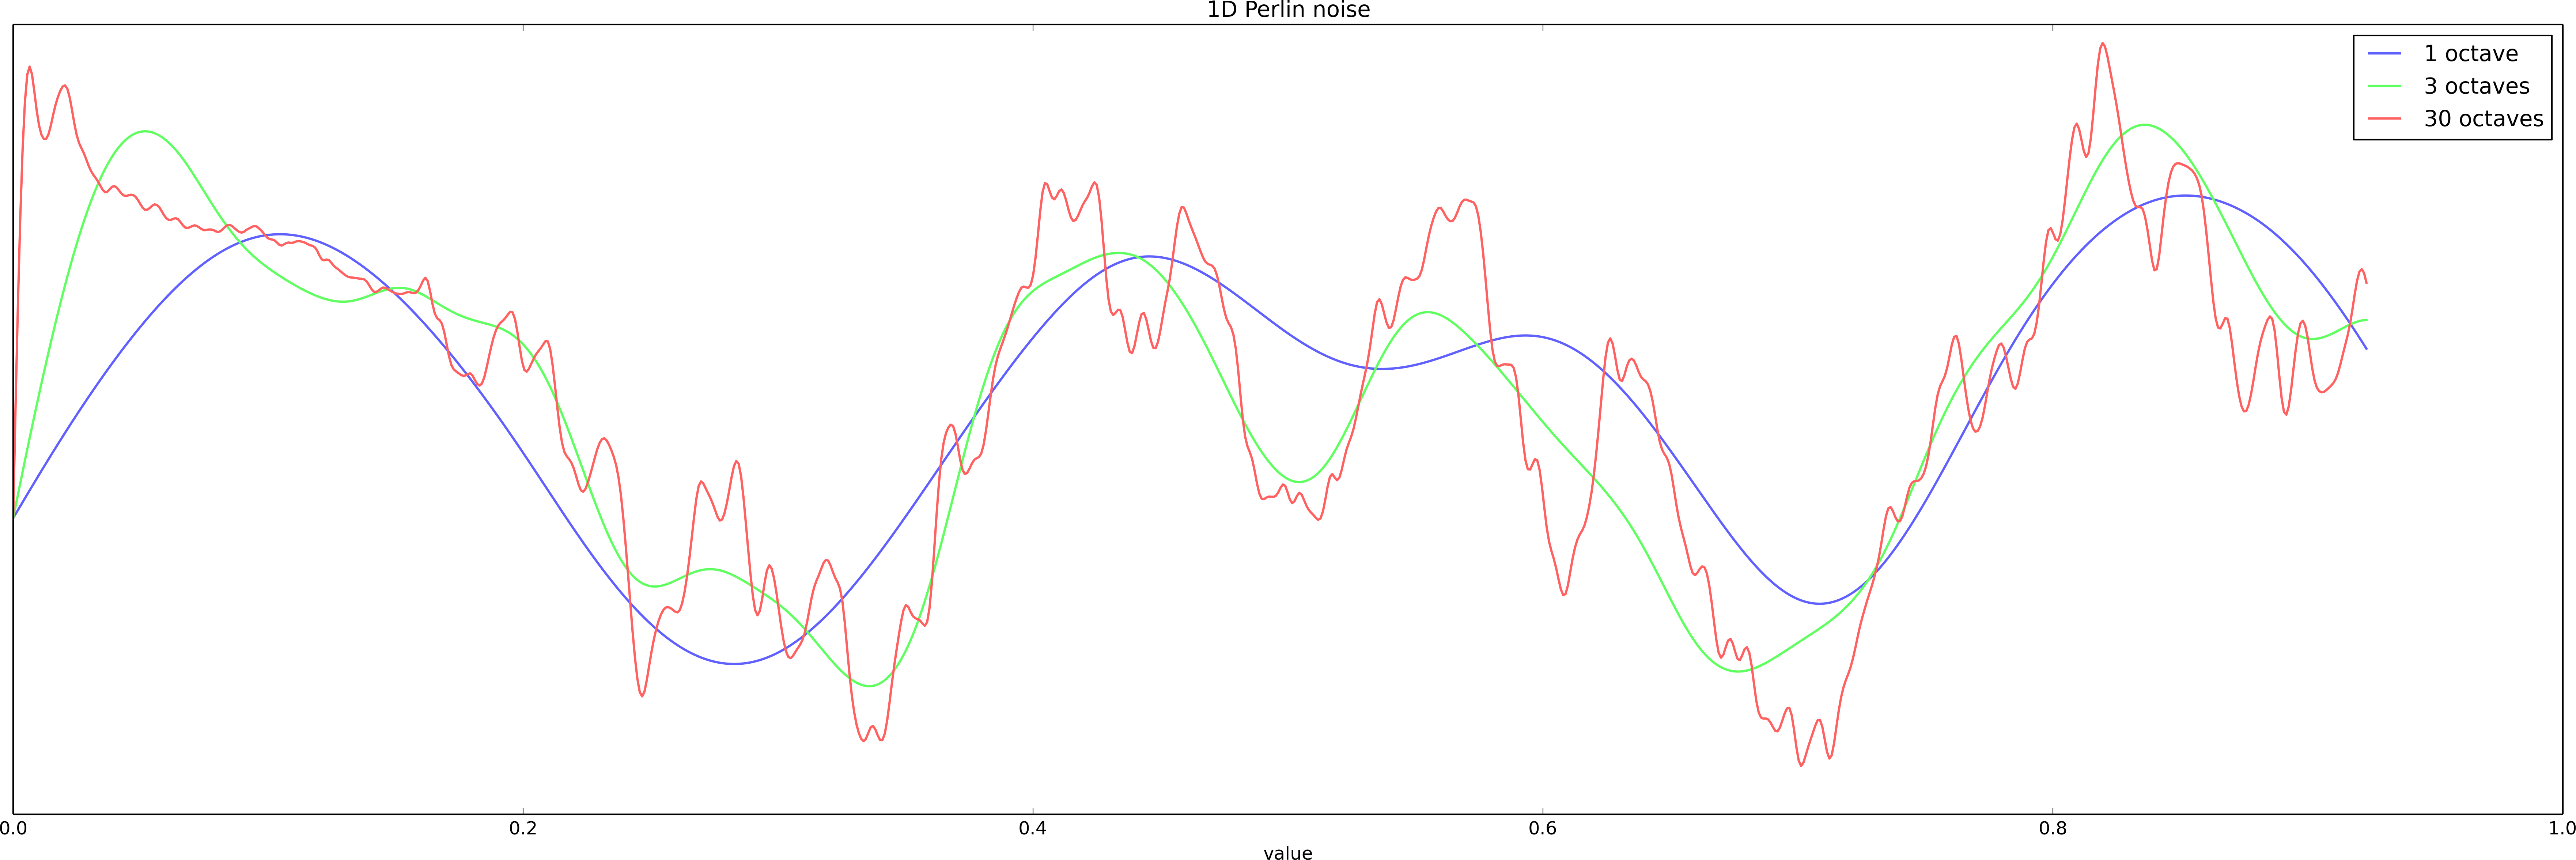
\includegraphics[width=.5\textwidth]{1d_perlin.png}
\caption{1D simplex noise with 1 (blue), 3 (green) and 30 (red) octaves. }
\label{fig:1dperlin}
\end{figure}


\section{Model}
In this paper, we are interested in developing a model using simplex noise to reproduce nanoporous structures that are as statistically close to actual simulations of porous media. For a given data set and a model, we wish to estimate the parameters that best represent the data. This is performed through a full likelihood analysis, where we in addition validate the model by comparing the radial distribution function $g(r)$, porosity and surface area of the system. The simulated system is confined to a cube of size $\SI{159}{\angstrom^{3}}$, but since the procedural noise function is continuous on all scales, the box could be of arbitrary size. 

\begin{figure*}
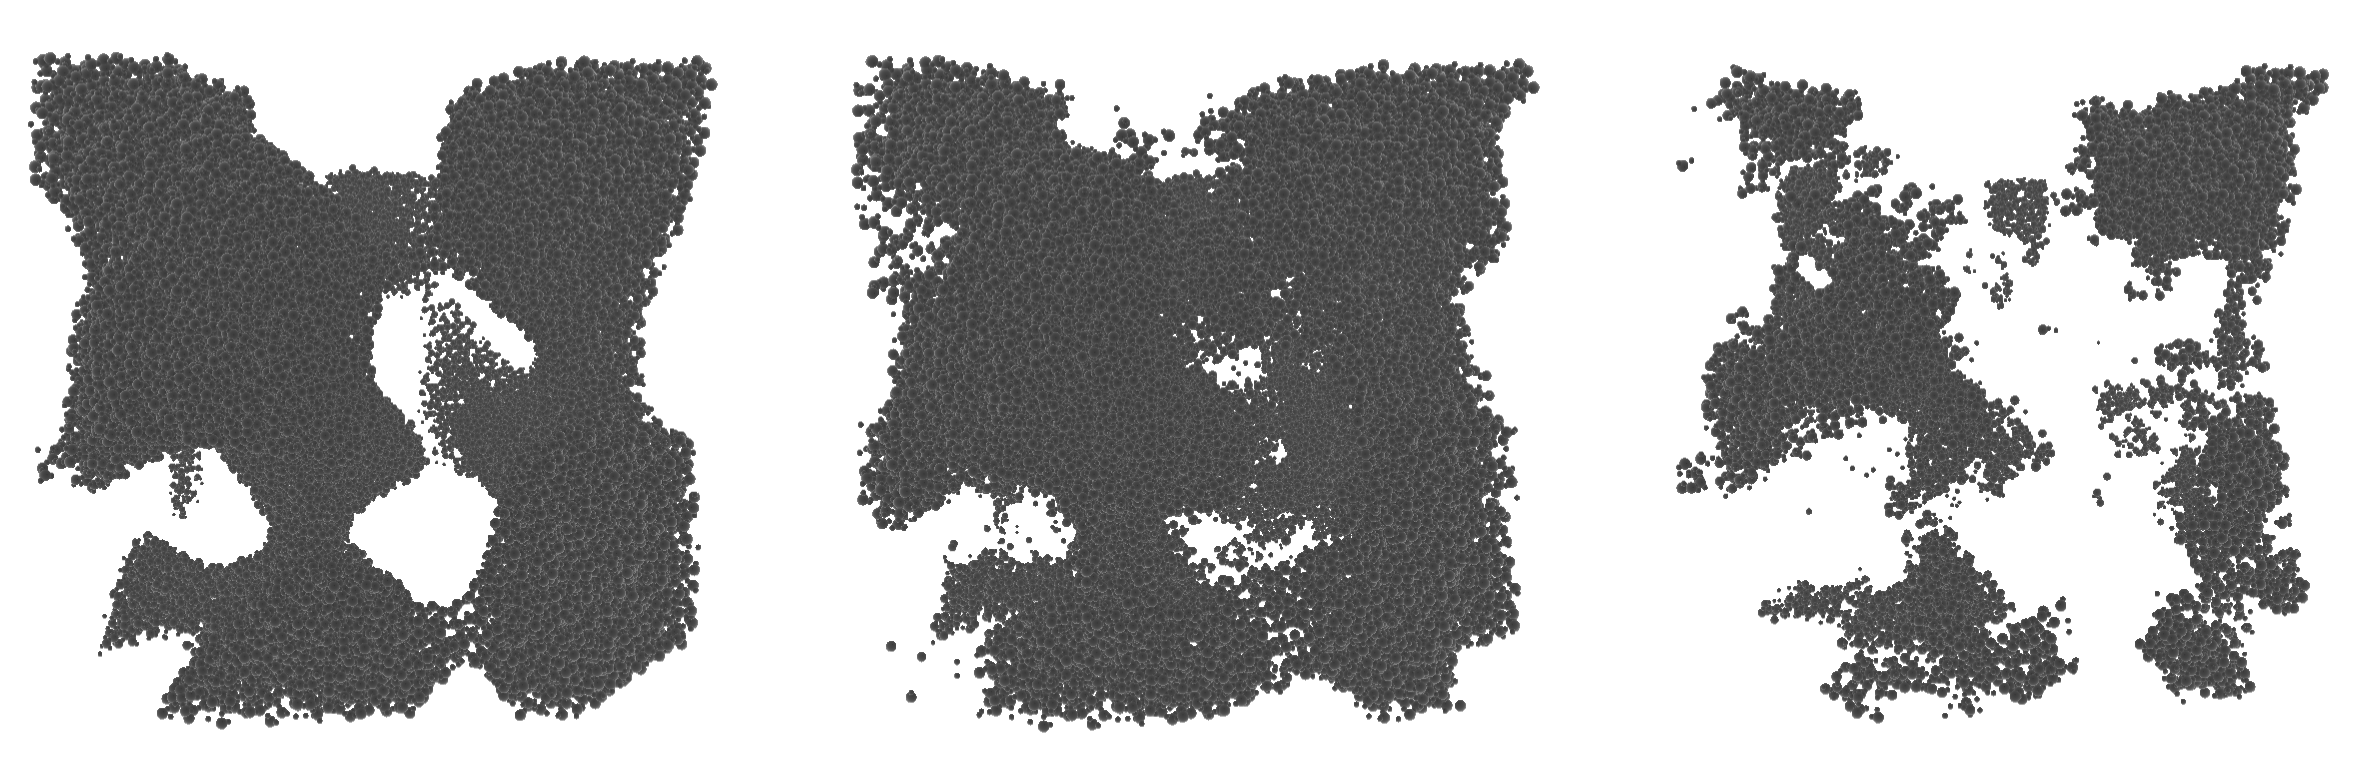
\includegraphics[width=.95\textwidth]{model_examples.png}
\caption{Examples of 3D simplex noise structures in nanoporous media. Left image: low persistence (large scale dominates), middle image: medium persistence (small scales starts dominating) and right image: high threshold (more atoms are discarded). }
\label{fig:model_example}
\end{figure*}
We construct a generic sum over procedural noise octaves with the expression: 
\begin{equation}
  M_1(\bar \theta) = M_1(\vec x, \psi, \Omega, \nu) = \sum_{\omega=0}^{\Omega} \psi^{\omega -1}   N\big((\vec x + \sigma \cdot \omega)\nu \cdot 2^{\omega-1} \big),
\label{eq:noisemodel1}
\end{equation}
where $\Omega$ is the total amount of octaves, $\psi$ the persistence (scale falloff), $N$ a generic $N$-dimensional noise function, $\sigma$ a predefined random vector that removes anisotropic artefacts and $\nu$ the frequency modifier representing the initial largest scales in the model. For simplicity, $\bar \theta$ here denotes the set of model parameters. For each mode, the frequency is thus multiplied, while the overall amplitude is damped by a given persistence. In the end, we simulate a large set of bulk particles without any walls, and use the noise function to remove particles that are not in a procedural void given by a threshold $\tau$. Three examples of this model are depicted in figure \ref{fig:model_example}, where we have used $\Omega=6$ octaves and the scale is $\nu=0.01$ and cut-off $\tau=0$. The left image depicts low persistence ($\psi = 0.0$), where only the first octave dominates (corresponding to large scales). The middle picture shows the same parameters with a higher persistence $(\psi = 0.5)$, where smaller scales become more dominating. In the rightmost picture, the effect of the cut-off threshold $\tau = -0.3$ is shown.   


\subsection{Model Measure}
In order to perform data analysis on the model parameters, we developed a code that uses Monte Carlo Markov chains in order to produce samples for building the likelihood. Before doing so, we need a model measure - a quantitative method that characterizes the internal structure of the porous media. This quantity should be computed for both the original data set and the one produced by our noise model. 

Ideally, the model measure should pick up all geometrical properties that are relevant for the physical study of interest. For instance, transport in porous media heavily depends on the pore size distribution and porosity, whereas chemical reactons are sensitive to surface area. \todo{referanser, malthe?} In this paper, we choose to focus on the radial distribution function $g(r)$ as defined and implemented in LAMMPS \cite{plimpton1995fast}. $g(r)$ describes how density varies as a function of distance from a reference particle, picking up both the intramolecular and intermolecular structure. We have chosen to ignore the short range contributions of $g(r)$ since the pore geometry does not depend on the intramolecular structure of SiO$_2$, but only the density variations at larger distances. Hereafter, $g_d(r)$ denotes the RDF calculated from simulated or experimental data, while $g_{M(\bar \theta)}(r)$ represents the RDF based on the procedural noise model $M(\bar \theta)$, where $\bar \theta$ are the set of model parameters. 

The method used for calculating porosity of a media is defined as in \cite{gelb1998characterization}, and we obtain the surface area of a porous media by using marching cubes triangulation to sum the surface area of the generated triangles. As discussed in \cite{gelb1998characterization}, the definition of surface area is ill-defined in atomic simulations, because a definition of pore space is needed. In the marching cubes triangulation, we generate a voxelized grid, the scalar field, with values being the distance from the voxel center to the nearest atom. The isovalue threshold defining the surface is chosen to be \SI{2}{\angstrom}, large nough to have a dense pore matrix, but small enough to have most of the available pore space defined as such. The important note here is that the same definition of surface is being used in all compared systems. 

\todo{skriv litt mer om hvorfor vi velger g(r)}






%\begin{figure}[htb!]
%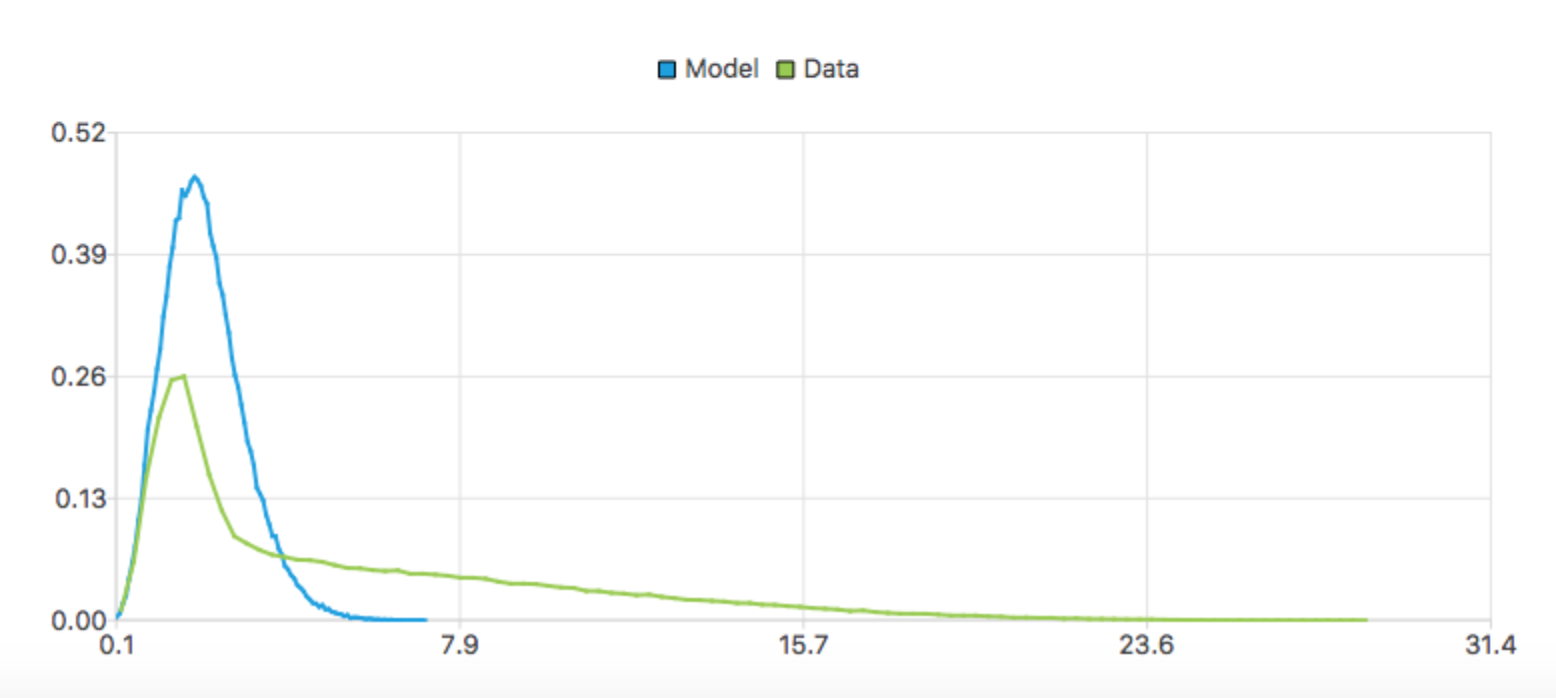
\includegraphics[width=.45\textwidth]{DTA.png}
%\caption{Distance-to-atom measure for two data sets with varying persistence. The green line corresponds to a mock data set with low persistence (dominated by large-scale modes), while the blue line corresponds to high persistence (dominated by small scale modes). }
%\label{fig:dta_example}
%\end{figure}



%\subsubsection{Fractal Dimension}
%The fractal dimension is a ratio providing a statistical index of complexity comparing how detail in a pattern changes with the scale at which it is measured. We provide a fracal

%\subsubsection{Octree Counting Measure (OCM)}

%\subsection{Diffusion Measure}

\subsection{Data analysis and the Likelihood}

The posterior probability is defined as the probability of the parameters $\bar \theta$ given the evidence $d$, or $P(\bar \theta | d)$. Bayes' theorem states that 
\begin{equation}
P(\bar \theta | d) = \frac{P(d | \bar \theta)P(\bar \theta)}{P(d)} \propto P(d | \bar \theta)P(\bar \theta),
\end{equation}
where $P(d | \bar \theta)$ is called the Likelihood $\mathcal L$ (the probability of evidence given parameters) and $P(\bar \theta)$ is the prior (the beliefs about the quantity before some evidence is taken into account). $P(d)$ is called the evidence, and is the probability of the observations (here assumed to be 1). Since the prior is a constant, we can therefore assume that the posterior distribution is proportional to the likelihood, or $P(d | \bar \theta) \propto \mathcal L$. In other words, to calculate the posterior and obtaining the best fit model parameters, we need only to estimate the likelihood function, which is connected to the $\chi^2$ by 
\begin{equation}
\mathcal L \propto e^{-\chi^2}.
\end{equation}


In order to test whether two 3D data sets are statistically equivalent up to the model measure $g(r)$, we calculate the $\chi^2$ between the two one-dimensional RDFs. Pearson's $\chi^2$ is defined as 
\begin{equation}
  \chi^2 = \sum_r \frac{ \Big(g_d(r) - g_{M(\bar \theta)}(r) \Big)^2}{g_{M(\bar \theta)}(r)^2},
\end{equation}
so for low values of $\chi^2$, the better the fit between data and model (up to $g(r)$). For a single-parameter model, we could simply just iterate over the lone parameter to obtain the minimum $\chi^2$ (where the best-fit parameter value is), however, with increased number of parameters comes increased computational cost. If we divide the parameter space into $N$ bins, the number of $\chi^2$ computations scales as $N^d$, where $d$ is the number of model parameters. To be able to build the full $\chi^2$ (and likelihood) parameter landscape, we there need to use Monte Carlo Markov chain methods (MCMC).

We are now interested in maximising the likelihood $\mathcal L$ as opposed to minimising the $\chi^2$, with the goal of mapping out the full $d$-dimensional likelihood space for the model parameters. We build the $d$-dimensional likelihood by letting random walkers traverse the parameter space guided by the MCMC test: for each step $M_n(\bar \theta)$ in parameter space, we calculate the likelihood for this parameter configuration. Then, we create a new set of parameters for the next step $M_{n+1}(\bar \theta)$ by choosing new parameters randomly from a $d$-dimensional sphere around the previous parameter composition. The model also selects a new random seed. We calculate the likelihood at the new step and perform the MCMC test: accept the new step if $\frac{\mathcal L_n}{\mathcal L_n+1} \ge 1$, or reject if the value is lower than a uniform random value $\in [0,1]$. 

Finally, we obtain the posterior $P(\bar \theta | d) \propto \mathcal L$ by building a $d$-dimensional histogram of the likelihood using the stored positions of the parameters. For a sufficiently large amount of steps, the MCMC algorithm ensures that the posterior converges to the likelihood, as long at the surface does not contain unreachable areas such as discontinuous patches or an infinite amount of maxima (as is the case for the function $f(x)=sin(\frac{1}{x}$). Luckily, as we shall see, the likelihood surface for our models tend to turn out with a single, well-defined maximum.  


\section{Results}
We now turn our attention to applying the MCMC framework on two kinds of data. First, we wish to test and verify the code by performing a full data analysis on mock data with known input parameters. This enables us to investigate the posterior distribution, and determine whether any potential problems could arise with the likelihood landscape, such as radom walkers trapped in local minima. We then continue with a full analysis of simulated SiO$_2$ data, and see whether the resulting best-fit parameter data set is consistent with the SiO$_2$ data set. 

\subsection{Model verification: Parameter estimation of mock data}
\begin{figure}[htb!]
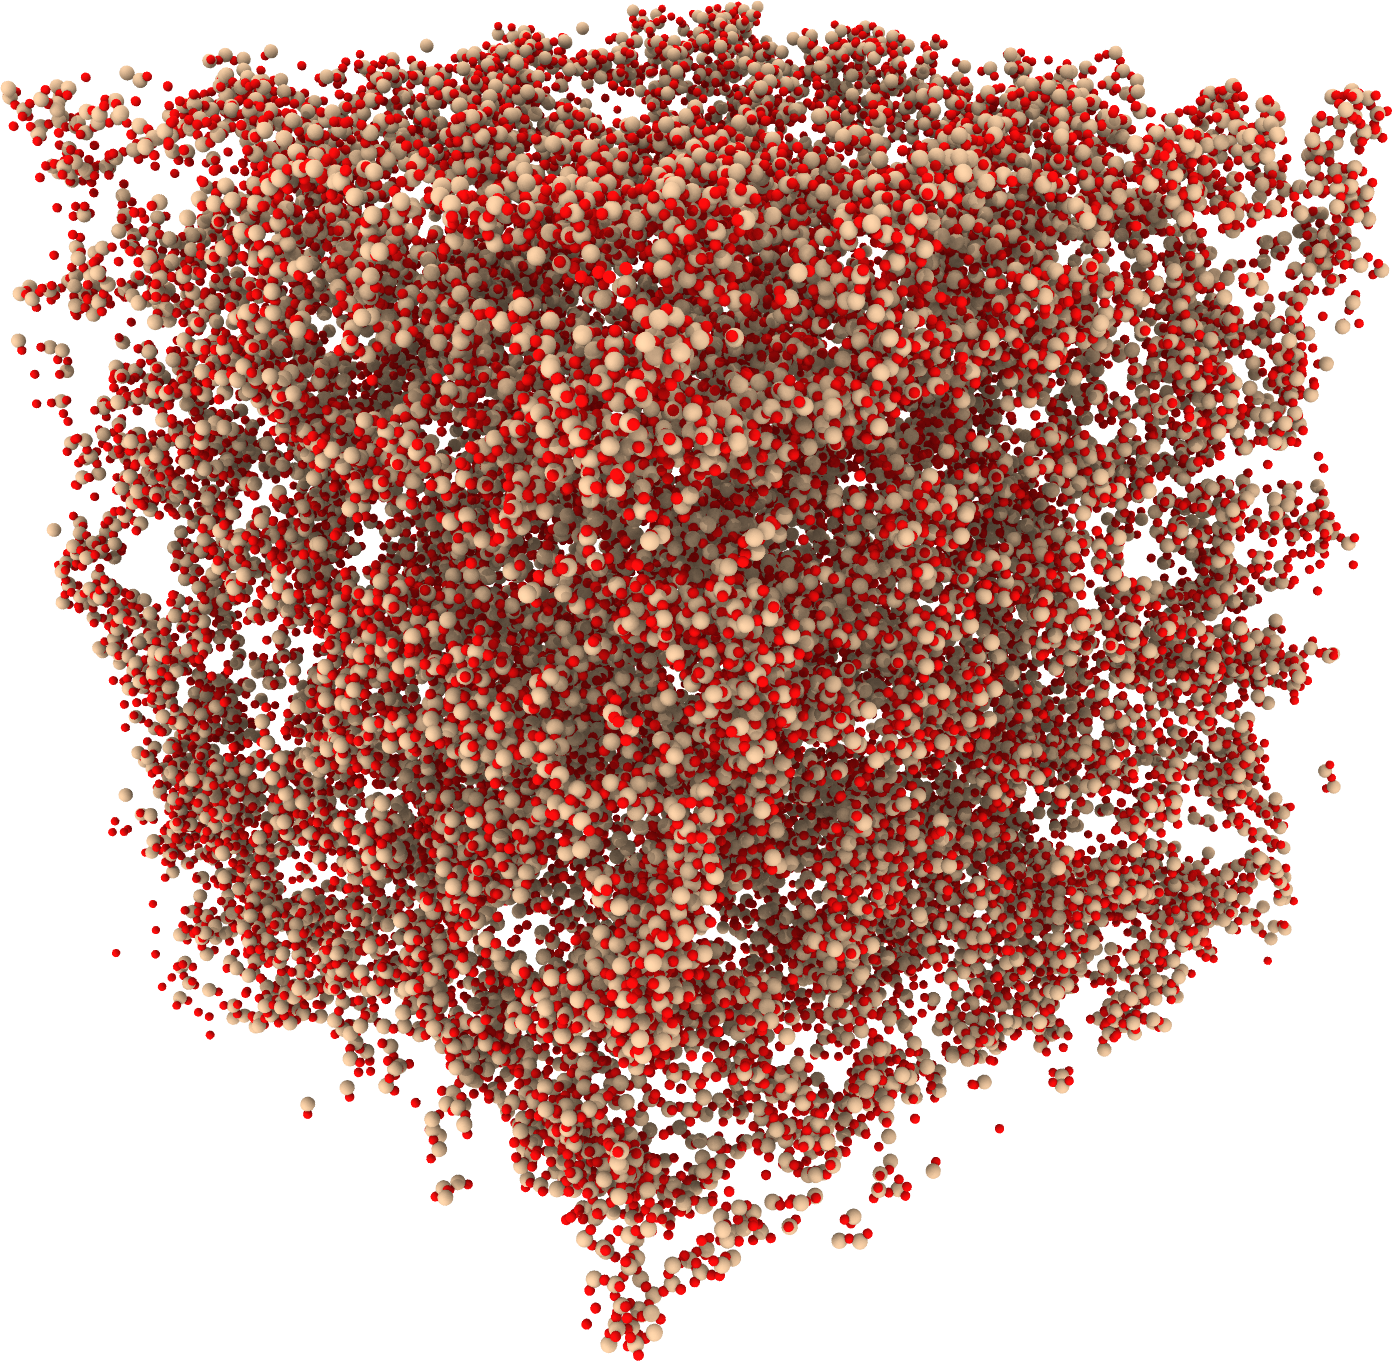
\includegraphics[width=.45\textwidth]{model_test.png}
\caption{Simulated mock data used for the initial model testing analysis. Input parameters are $\nu=0.03$,$\tau=-0.02$ and $\psi=0.6$.}
\label{fig:mockdata}
\end{figure}
In order to verify our likelihood code, we perform a model verification test on a mock data set with known input values. In this example, we only use standard simplex noise with three free parameters: the persistence $\psi$, threshold $\tau$ and scale $\nu$. We simulate a data set of $159 ^3 \AA$ of $\sim 255 000$ atoms, and perform the cut-off given input parameters $\Omega=3$, $\Psi = 0.6$, $\tau=-0.2$, $\nu=0.03$. The resulting 3D structure is depicted in figure \ref{fig:mockdata}. 

We continue by performing a full MCMC analysis of the mock data with using a parallelized code running on a 48 core cluster. In order to produce 300 000 samples, about 48 hours was needed. The results from this analysis can be seen in figure \ref{fig:mockdataresults_pts}, where the upper panel depicts the marginalised 1D posteriors while the lower shows the marginalised 2D posteriors. The centre and left image shows that the input parameters of $\tau=-0.2$(threshold), $\psi=0.6$(persistence) and $\nu=0.03$ are all reproduced well within $1 \sigma$.

Note that there seems to be no problems with the posterior distribution in terms of local minima or multiple maxima. 

\begin{figure*}
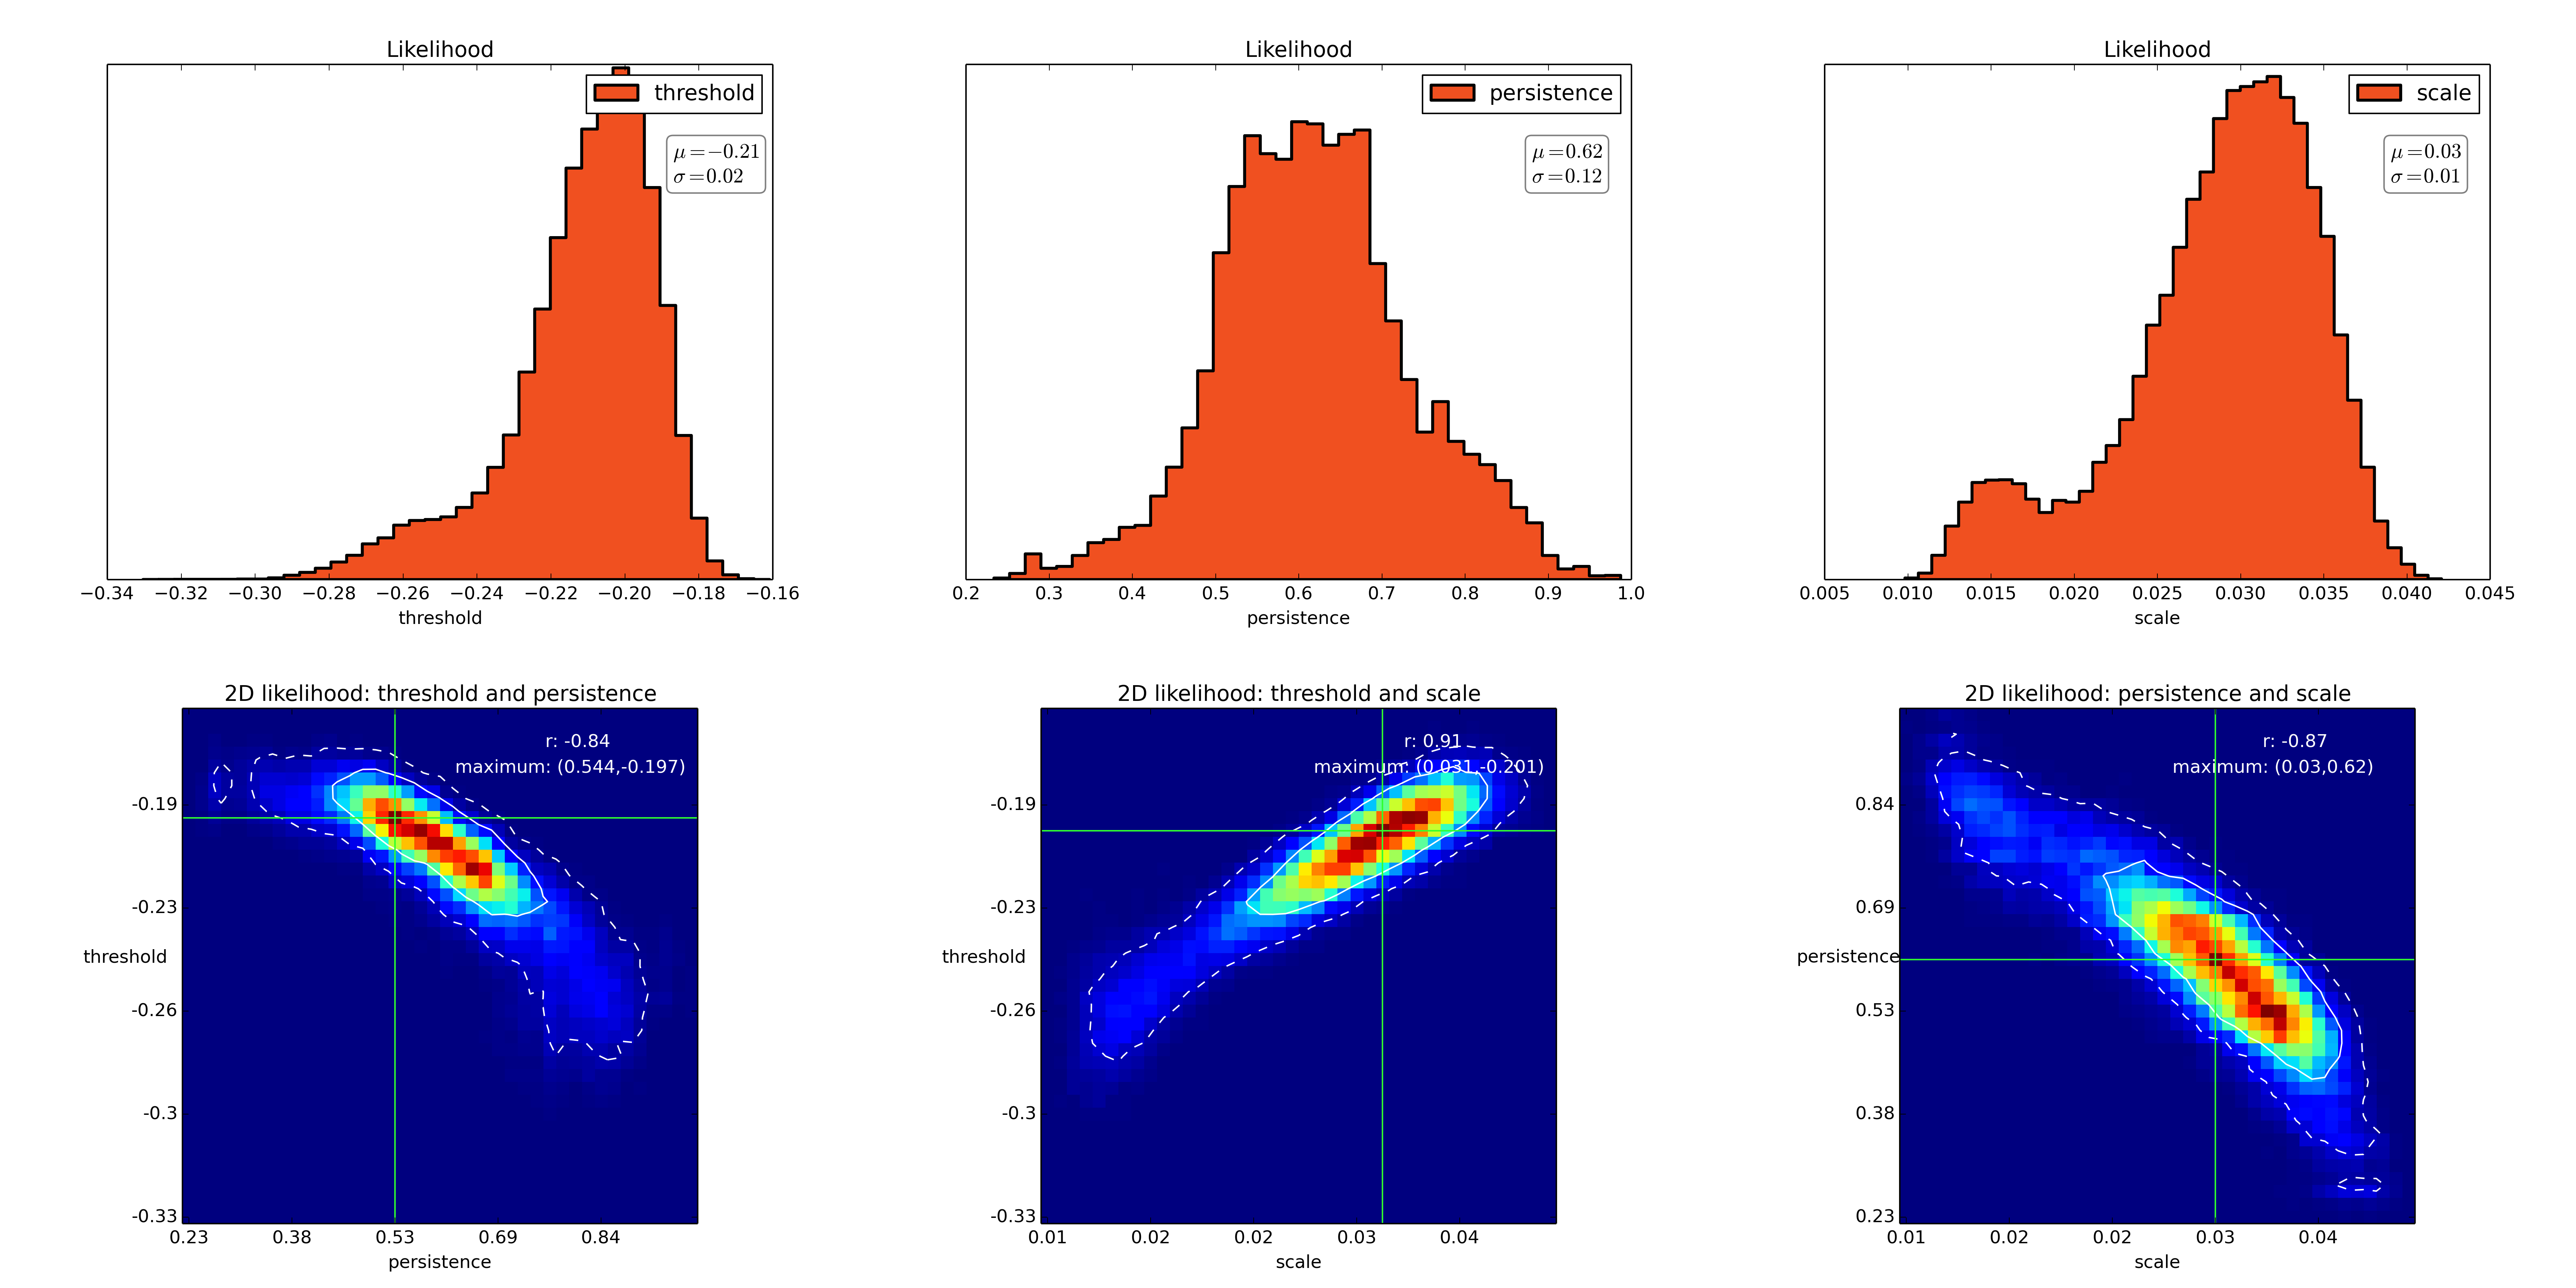
\includegraphics[width=.99\textwidth]{mock_data_results_pts.png}
\caption{Results from the model validation simulation. The upper panel displays the marginalised 1D posteriors for each parameter, while the lower panel depicts the marginalised 2D posteriors. Note that all input parameters were reproduced well within $1\sigma$ (inner contour line).}
\label{fig:mockdataresults_pts}
\end{figure*}

\subsection{Parameter estimation of simulated nanoporous silica}
%\begin{figure}
%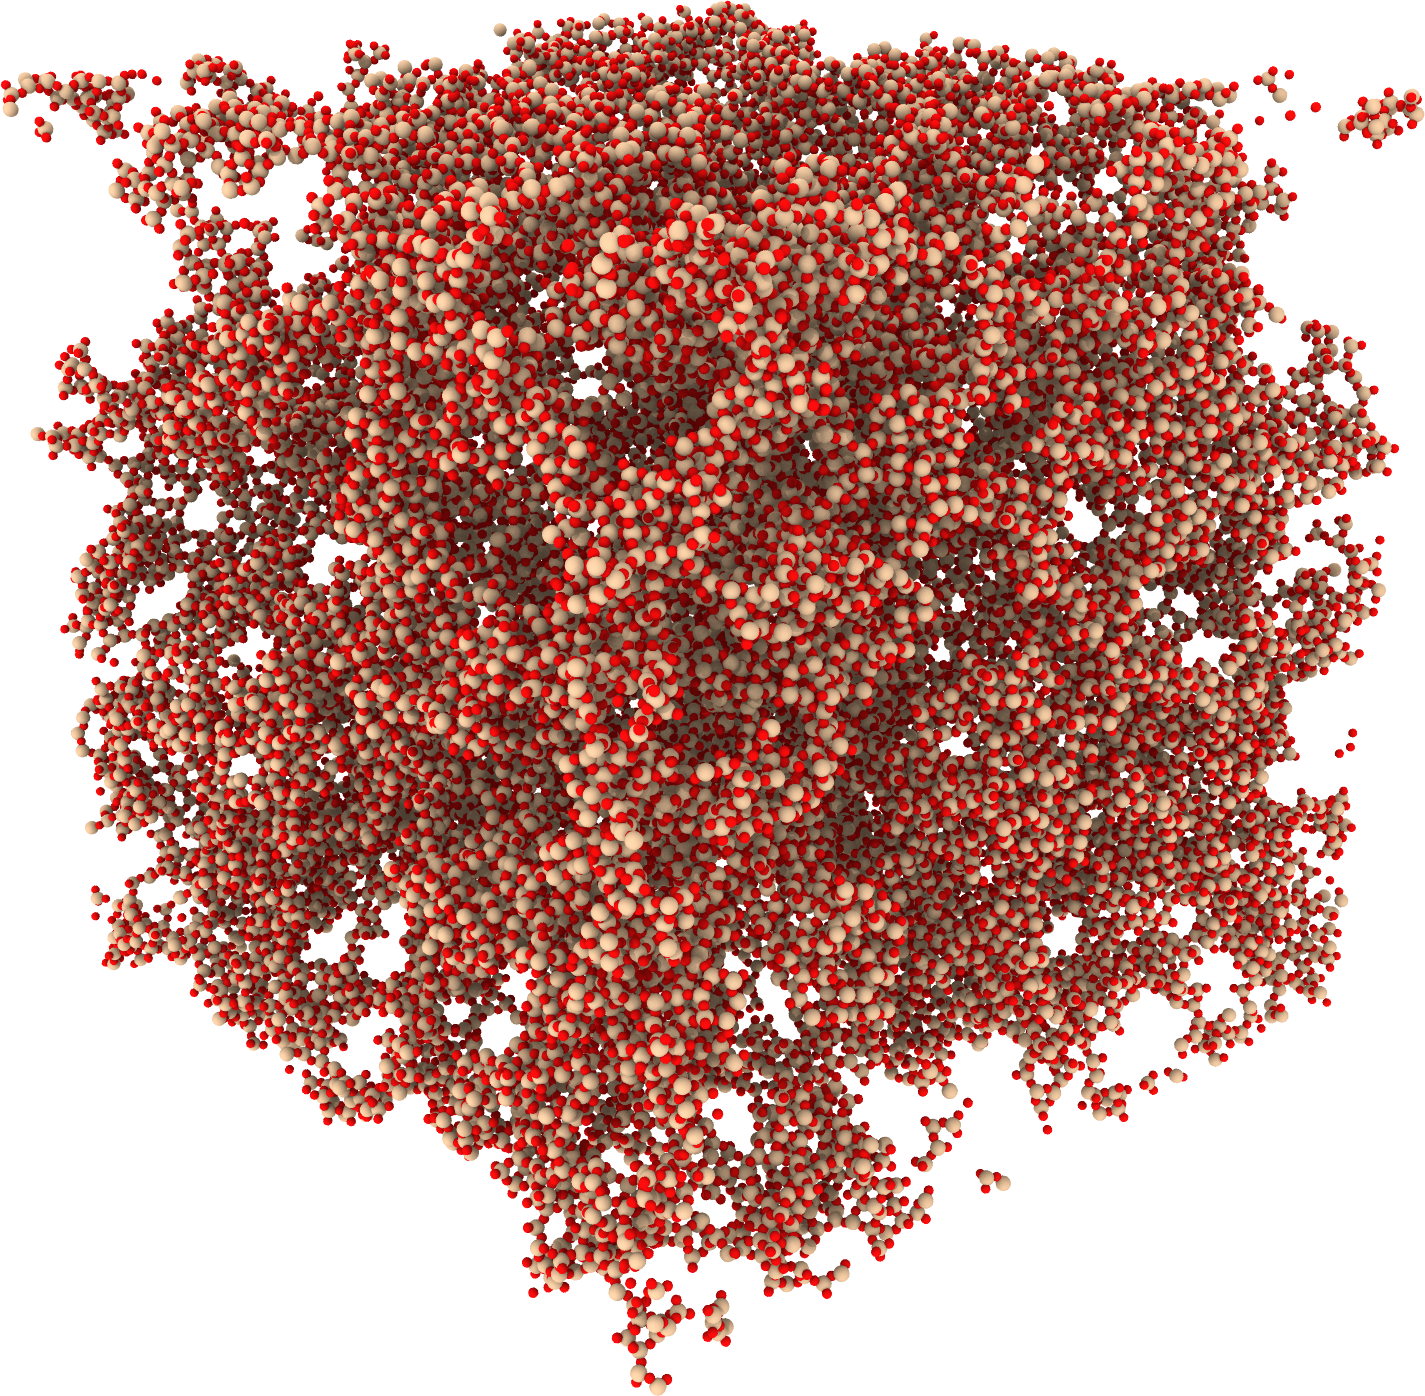
\includegraphics[width=.49\textwidth]{sio_porous.png}
%\caption{Simulated silica created with LAMMPS. The box is $159^3 \AA$, with $100 000$ particles, having been created by cooling an expanding system until quenching was achieved. Note the similarities between the pores here and in figure \ref{fig:mockdata}.}
%\label{fig:si2data}
%\end{figure}
\begin{figure*}
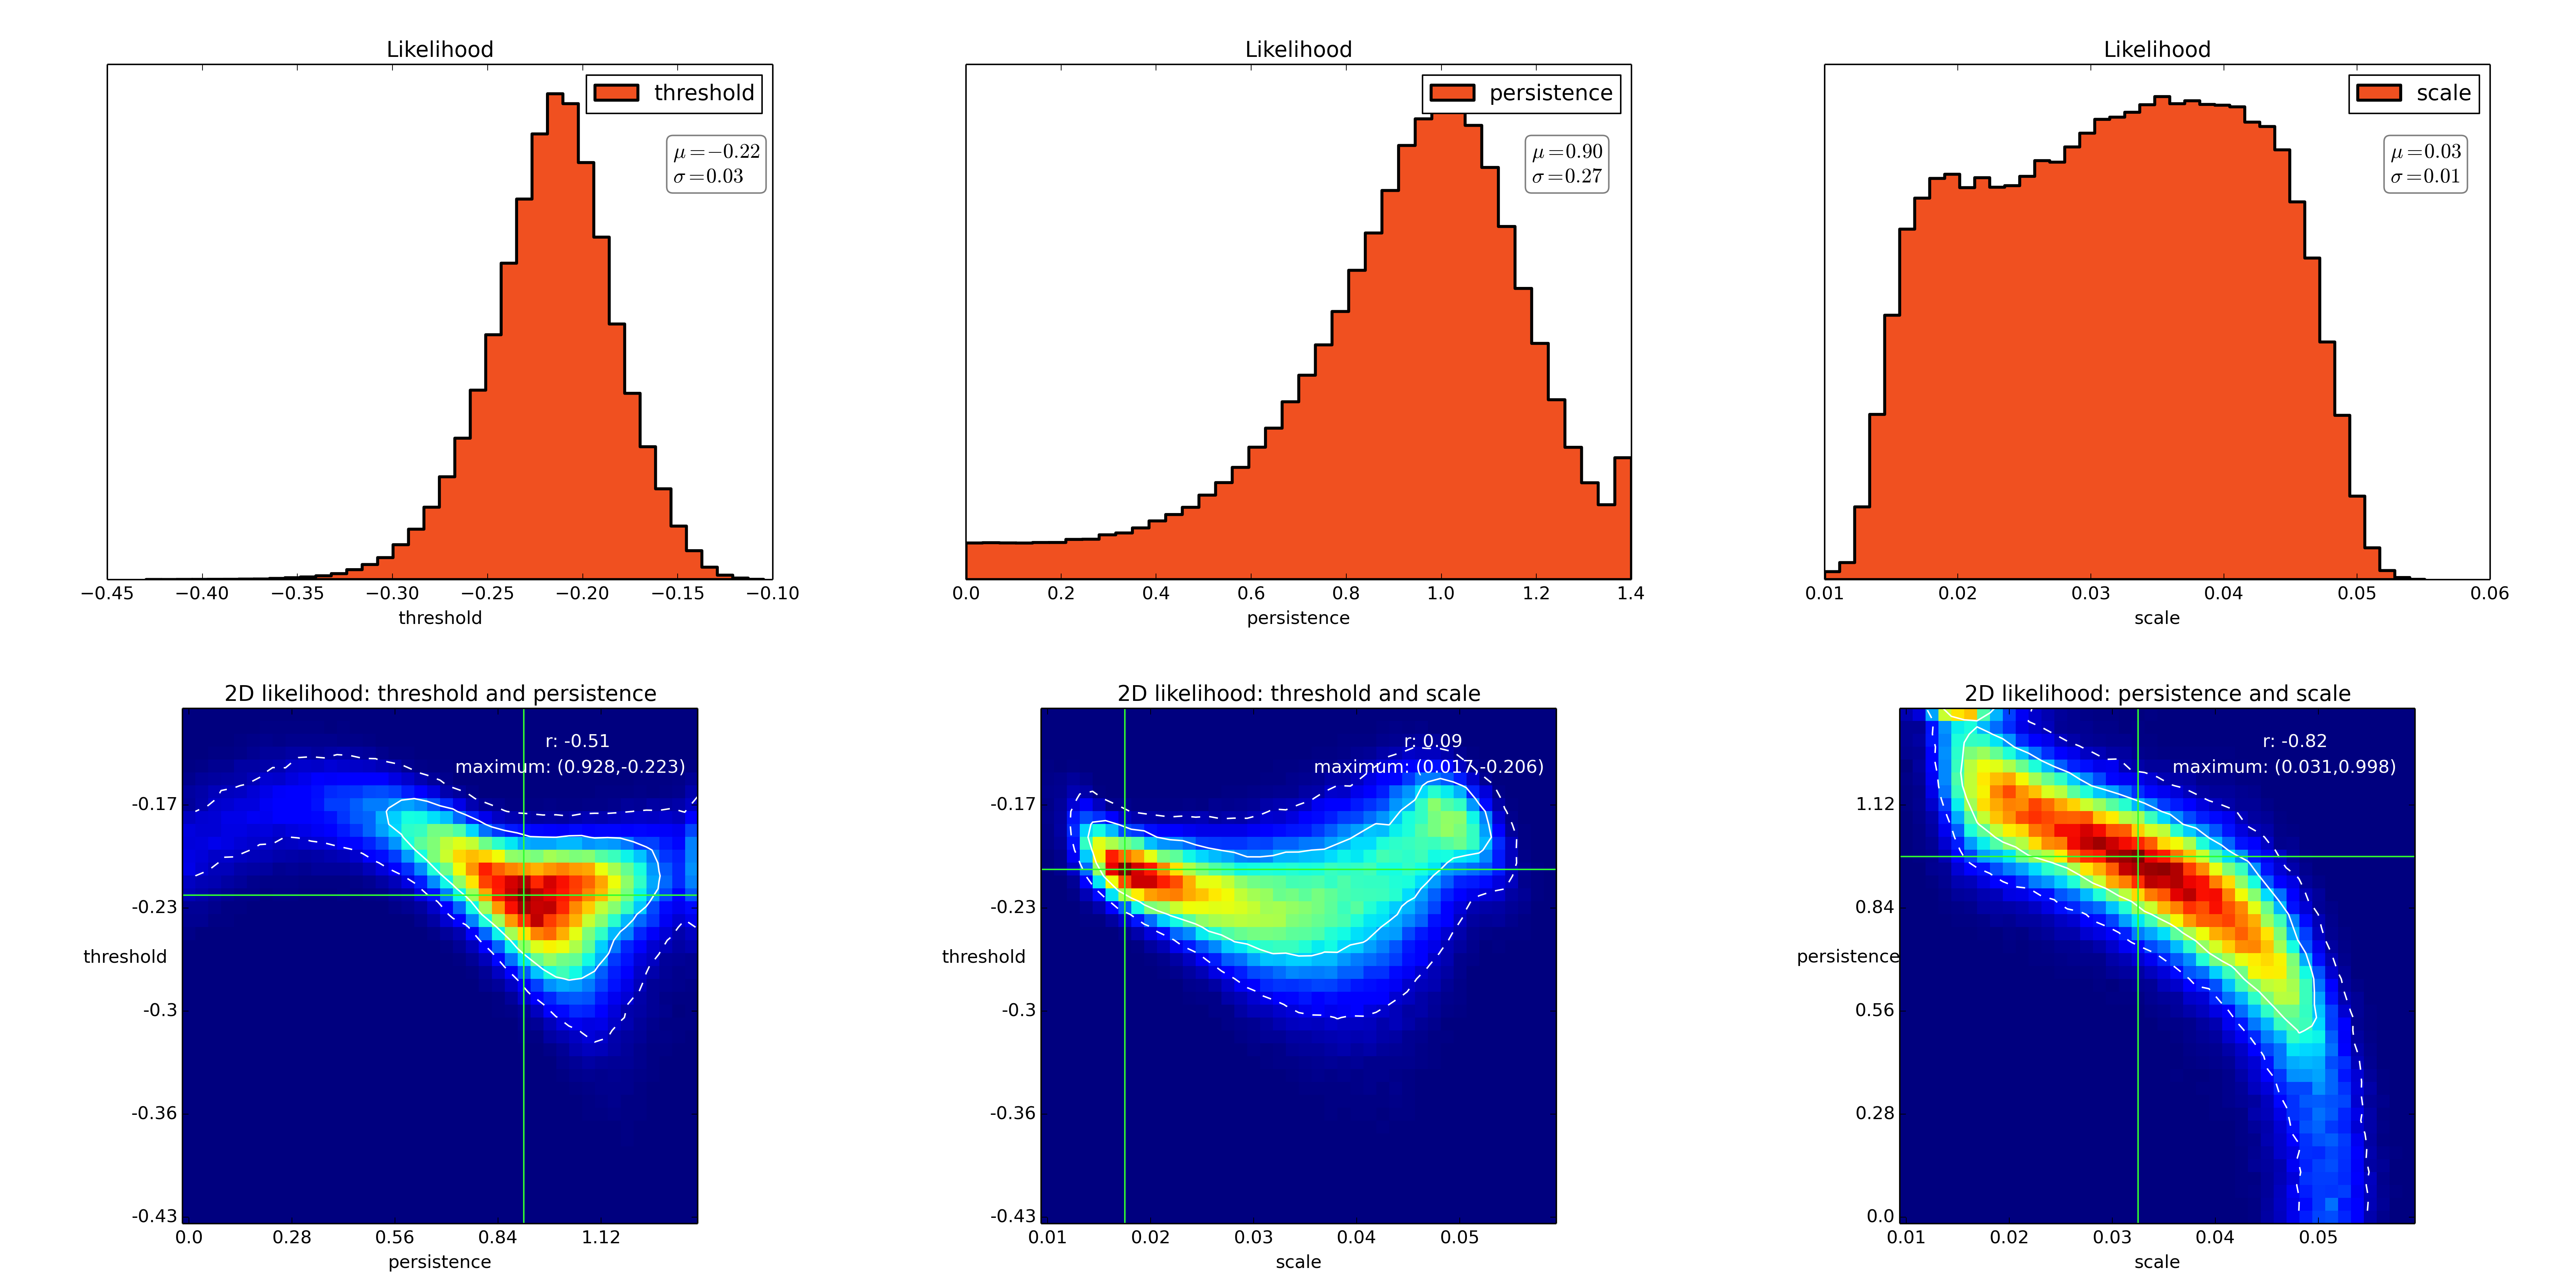
\includegraphics[width=.99\textwidth]{results_porous_full.png}
\caption{Results from the analysis of a simulated $159^3$ \AA SiO$_2$ nanoporous data set. The upper panel displays the marginalised 1D posteriors for each parameter, while the lower panel depicts the marginalised 2D posteriors. Best fit parameters from the maximum 3D likelihood suggest $\tau=-0.2$, $\psi=0.8$ and $\nu=0.3$.}
\label{fig:porous_results1}
\end{figure*}

We now perform a parameter fitting analysis on realistic simulated nanoporous media. Using LAMMPS \cite{plimpton1995fast} and the Vashishta-potential \cite{vashishta1990interaction}, we simulate system consisting of $14^3$ betacristobalite unit cells of SiO$_2$, corresponding to system size of approximately \SI{100}{\angstrom}. The temperature is then increased to \SI{4500}{\kelvin} using NVT integration. After an initial period, we expand the box to \SI{159}{\angstrom} to achieve a porosity $\phi=0.75$. Then, the system is quenched by setting the temperature to \SI{300}{\kelvin}, resulting in the nanoporous media on the right side in figure \ref{fig:porous_vs_model}. By choosing a different seed for the initial velocities, it is easy to produce other samples.

With the model described in equation \ref{eq:noisemodel1}, we perform a full likelihood analysis of the data set with the three free parameters $\tau$, $\nu$ and $\psi$ using $g(r)$ as the measure. The resulting marginalised posteriors are depicted in figure \ref{fig:porous_results1}, with best-fit parameters $\tau=-0.2$, $\psi=0.8$ and $\nu=0.3$ is extracted from the full 3D likelihood. We also display $g(r)$ for the input data set, a best-fit parameter data set and a bad-fit data set in figure \ref{fig:gofr1}, to illustrate the sensitivity of $g(r)$ given the model parameters. Note that we are not able to accurately reproduce the structures of the SiO$_2$ $g(r)$ with our current model, but hope that we during future work will be able to produce another model that provides a better fit with this measure. 

Note that the surface atoms are not in chemical equilibrium since some neighbors of a surface atom might have been removed. In order to use the generated geometry in molecular dynamics, one would need either noble gas atoms which may be stable, or apply passivation step.

\begin{figure}
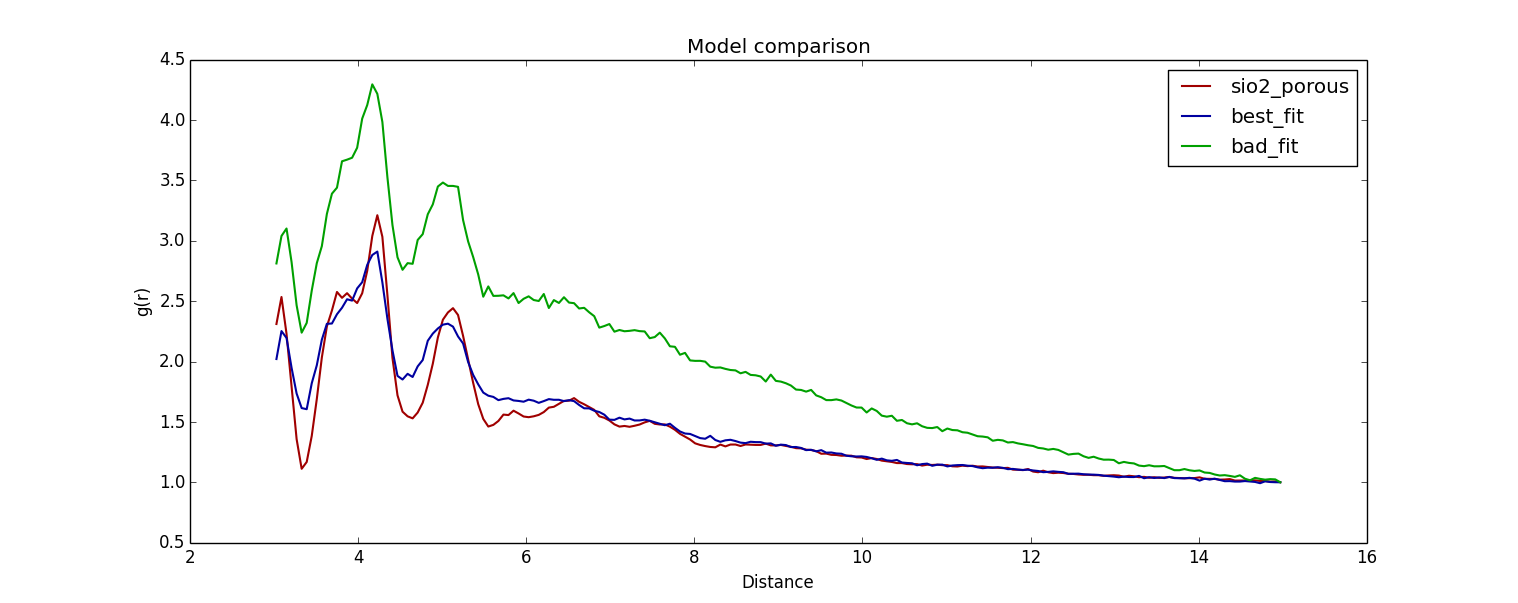
\includegraphics[width=.45\textwidth]{gofr_plot.png}
\caption{$g(r)$ for three data sets: the simulated SiO$_2$ input data set (red), the best-fit parameter model (blue) and a random low-fit parameter model (green). \todo{Bytt denne figuren med VMD sin beregning. Normaliseringen vår er gal.}}
\label{fig:gofr1}
\end{figure}
Finally, we depict a comparison of the actual simulated input SiO$_2$ data set together with a representation of the best-fit parameters in figure \ref{fig:porous_vs_model}   
\begin{figure}
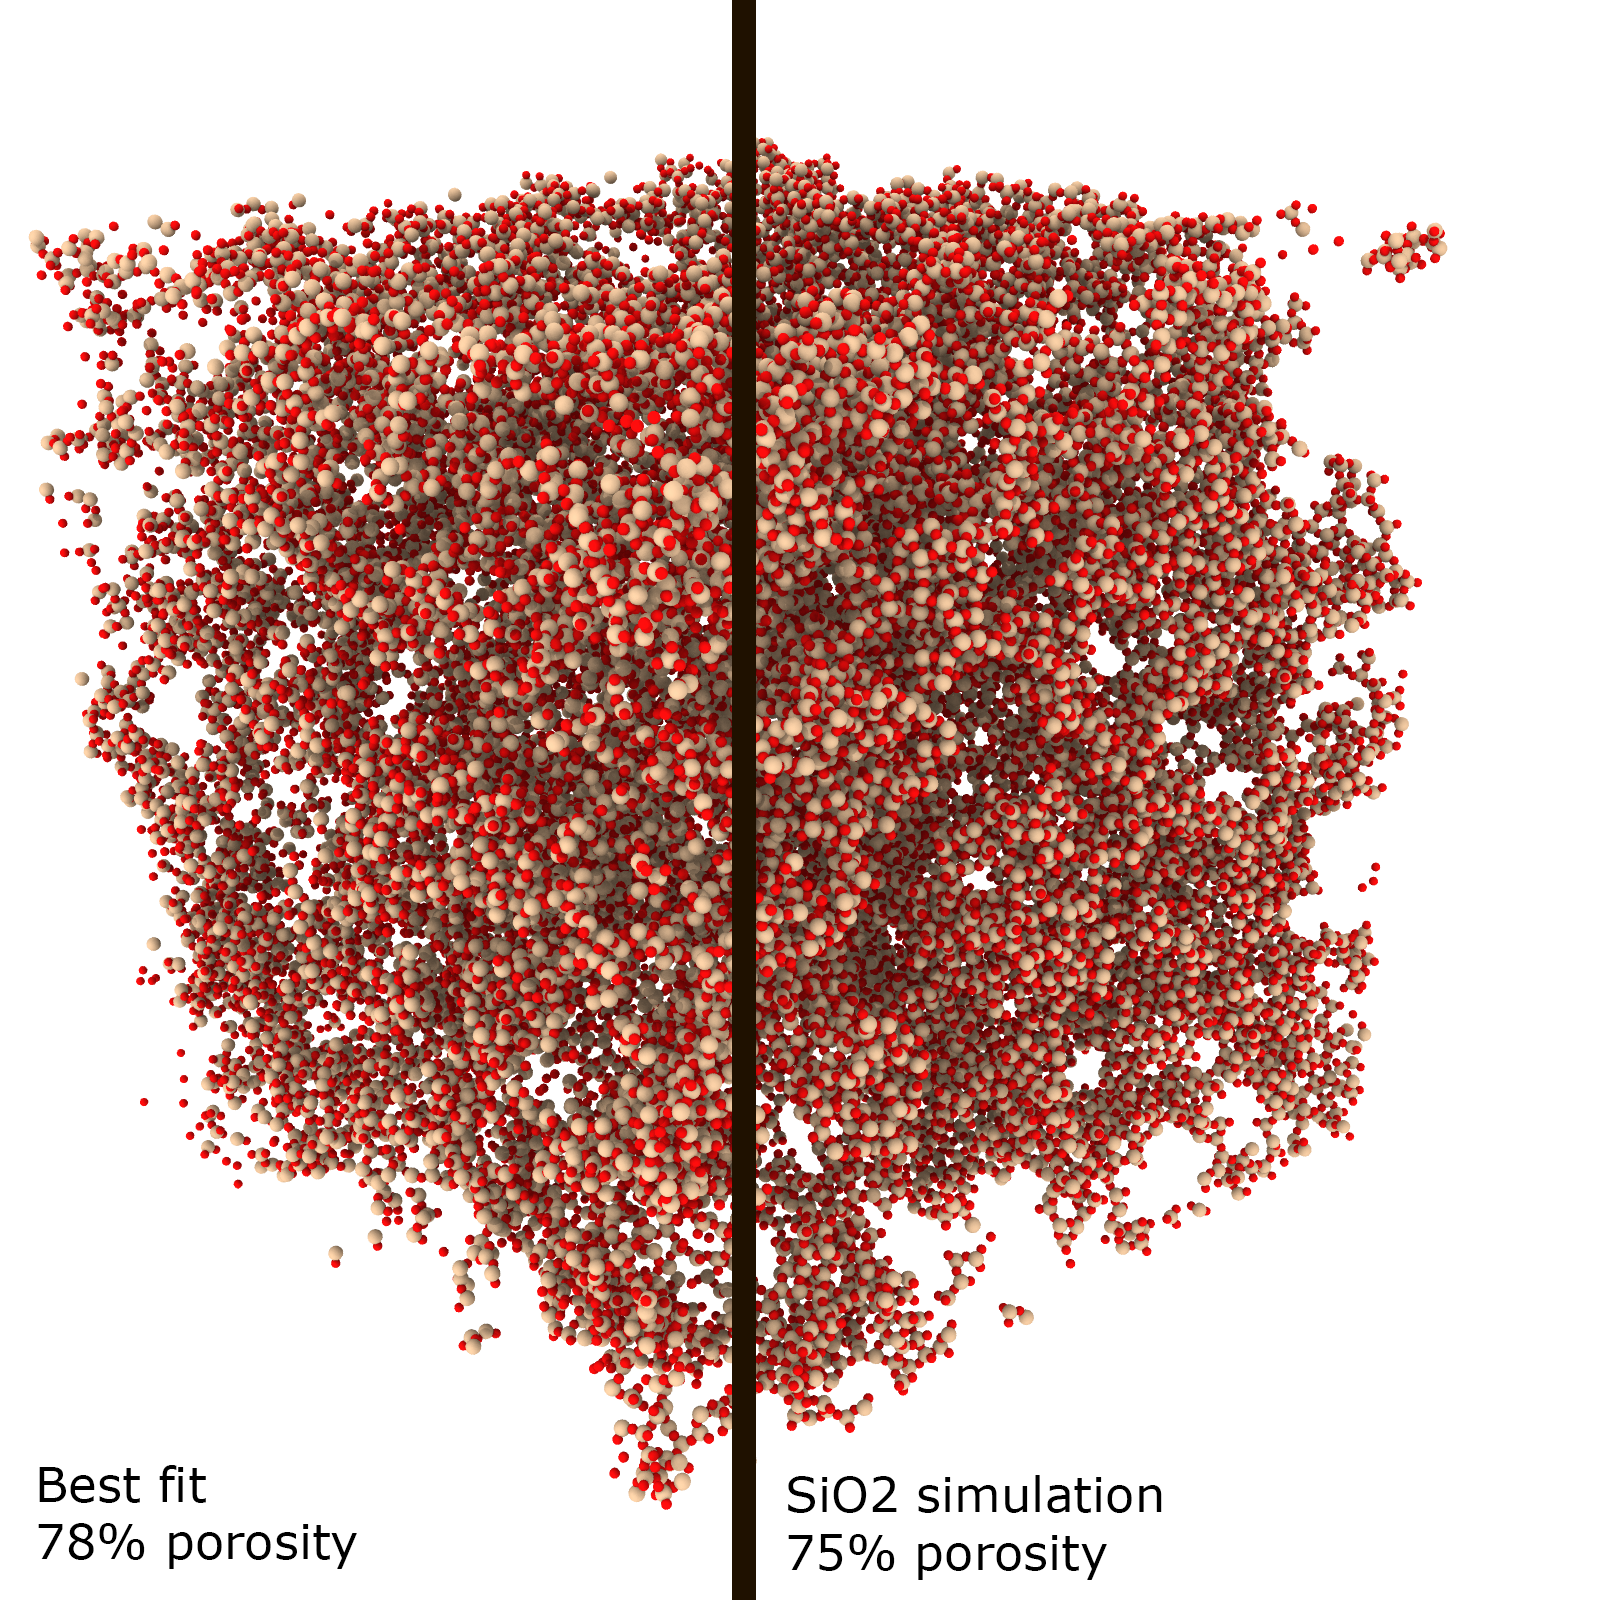
\includegraphics[width=.45\textwidth]{comparison.png}
\caption{Right side: A realisation of the best-fit parameters $\tau=-0.2$, $\psi=0.8$ and $\nu=0.3$. Left side: Simulated SiO$_2$ input data set used for parameter estimation. Although the pore geometry seems to be similar, we see some artifacts, such as single loose atoms in the generated geometry.}
\label{fig:porous_vs_model}
\end{figure}

The porosity of the input SiO data set is $75\%$, while the best-fit data set has porosity $77\% \pm 3 \%$, depending on the random seed. In addition, the surface area of the original data set was $\sim \SI{29000}{\angstrom^2}$, while the best-fit data shows similar values with surface are ranging between $\sim \SI{28000}{\angstrom^2}$ and $\sim \SI{30000}{\angstrom^2}$.
\todo{legg ved 3D plot av likelihood for aa vise at den er kjekk og fin}

\subsection{Some notes on the results}
It is worth to note that since we are chiefly interested in obtaining a set of parameters that reproduces a statistical correct representation of the input data, we are relatively free to choose parameters as desired. In the previous analysis, we selected a best fit threshold value of $\tau=-0.2$, but from the width of the likelihood it is clear that nearby parameters would also be suitable. However, the surface area is strongly correlated with this value, so even slight deviations (e.g. $\Delta \tau = 0.05$) yields a relatively large change in surface area. 

In addition, we do not claim that this model accurately reproduces the pore structure observed in nanoporous simulations, as is evident from the RDF shown in figure \ref{fig:gofr1}.

\subsection{$g(r)$ variation}
We also calculated the variation in the $g(r)$ given initial conditions on both our model and simulated data. In terms of the data, the variation is attributed as the initial velocities of the particles in the LAMMPS simulation. For the model, it corresponds to the random seed. We found that varying these initial conditions have negligible effect on the calculation of $g(r)$.


%persistence : 0.875111019125
%scale : 0.036638
%threshold : -0.236784875   78% porosity

% bad fit : scale 0.1, p = 1, threshold = -0.3


\section{Conclusion}
\todo{konklusjon maa renskrives}
In this paper, we have proposed a novel method for generating a simple kind of nanoporous media using procedural methods, namely simplex noise. We have developed tools for creating such porous materials, and also estimating model parameters given data. We have shown that it is possible through a full likelihood analysis to reproduce the input parameters of a simulated model. In addition, we performed an analysis on a simulated $159^3 \AA$ data set of SiO$_2$, and explain that while porosity and surface area corresponds well between the model and data, the $g(r)$ shows that the current model does not exactly reproduce correct data. However, we do not claim that the current model should do so yet, since we have chosen the simplest kind of summation with regards to procedural noise modes. 

\subsection{Future work}
In this paper, we have only considered the simplest kind of procedural noise: a simple sum over modes with threshold cut-off $\tau$, scale fall-off persistence $\psi$ and initial scale $\nu$. We have also seen that, even through both porosity and surface area accurately reproduced, there are features in the RDF that are not fully captured with the current model. This is evident from the images of the simulated structure seen in figure \ref{fig:porous_vs_model}, where the connecting nearly one-atom thin walls are difficult to reproduce with the current model. However, as procedural noise exert properties closely related to that of fractals, it is possible to extend the number of parameters and define new models with very different properties. Some examples of these models are depicted in figure \ref{fig:future_models}, where the left- and centre images show a new model with two new parameters (offset and gain), while the rightmost panel shows a simulation where the scale $\nu$ is itself being perturbed by procedural noise, yielding strong circular asymmetric patterns.   

Another immediate application would be to estimate model parameters given experimental observations of porous media. This would enable us to estimate new parameters such as instrumental noise, deviations from symmetry (yielding asymmetric properties) and pureness of samples. In addition, by analysing just a few samples and producing an accurate model, we are able to produce an arbitrary amount of statistically correct samples, free from instrumental noise and artefacts. 

A final key analysis would be to compare properties such as permeability through finite-element simulations of gas/liquid flow through our simulated structures, in addition to exerting shear forces, and comparing with actual simulated data from e.g. LAMMPS. Since the noise function is a continuous boolean function that only checks whether a position is within a wall or void given a threshold, we are not limited to any size of the simulated system, and simulated particles traversing the media has arbitrary range.  


%Minkowski functionals and topology, genus etc

%Swiss noise

\begin{figure*}
\includegraphics[width=1\textwidth]{future_models.png}
\caption{Example of future models. Left panel: A multi-fractal model with thin surfaces and large pores. Centre panel: a multi fractal with cave-like structures. Right panel: A model with strong asymmetric noise. }
\label{fig:future_models}
\end{figure*}

\todo{Kanskje fake-latin burde fjernes? Usikker!}
Ut hendrerit cursus libero, in scelerisque tortor sollicitudin accumsan. Nam eleifend velit metus, quis volutpat justo faucibus ut. Cras ut sem in nunc fringilla egestas vitae sit amet justo. Ut vel condimentum tortor. Morbi in massa in ipsum ultrices tincidunt. Duis feugiat dignissim nisi ac ultricies. Quisque eget risus fermentum, condimentum massa ullamcorper, posuere neque. Nam congue consequat mi, vel commodo mi tempus eget.

Nullam ultrices, velit sed venenatis ultrices, risus urna ultricies magna, at pretium lorem nibh et nunc. Suspendisse sed mattis leo. Nulla facilisi. Praesent finibus lobortis leo, ut porttitor massa tincidunt ut. Vivamus quis orci eu sem sodales ornare. Cras sed faucibus velit. Phasellus scelerisque mauris quis lorem dignissim vehicula. Sed tempor ut urna sed bibendum. Donec et nibh pulvinar, commodo magna ac, interdum nibh. Sed laoreet ipsum quis quam lacinia, in dictum erat laoreet. Etiam rhoncus mauris arcu, ac egestas lacus facilisis nec. Pellentesque a orci vitae felis faucibus ultrices sed non massa. In posuere vel ex in elementum. Aenean ac neque a enim gravida tristique eu ac lacus. Ut tincidunt venenatis lectus, et maximus mauris.

Proin ornare nulla id tristique placerat. Integer nec elementum tellus. Cras at tempus lectus. Cras lorem est, ornare id condimentum vitae, scelerisque eu lectus. Aenean libero arcu, consequat vel sagittis eget, sagittis ut neque. Pellentesque habitant morbi tristique senectus et netus et malesuada fames ac turpis egestas. Aenean nec quam sodales, mollis est sit amet, vulputate turpis. Praesent tempus diam eu sem laoreet finibus. Nulla finibus, sapien vel lobortis ultricies, mauris ipsum aliquet urna, quis rutrum sapien dui id ipsum. Quisque sodales ex sapien, ac egestas lacus suscipit et. Suspendisse accumsan rhoncus tristique. Pellentesque ut eros lectus. Praesent viverra sit amet odio nec vulputate. Class aptent taciti sociosqu ad litora torquent per conubia nostra, per inceptos himenaeos. Nulla molestie metus vitae libero vulputate, at interdum enim tempus.



%%%%%%%%%%%%%%%%%%%%%%%%%%%%%%%%%%%%%%%%%%%%%%%%%%%%%%%%%%%%%%
%%%%%%%%%%%%%%%%%%%%%%%%%%%%%%%%%%%%%%%%%%%%%%%%%%%%%%%%%%%%%%
\bibliography{bibliography}

%\begin{thebibliography}{9}

%\bibitem[Groeneboom2014]{groeneboom2014} Groeneboom, N.~E., \& Dahle, H.\ 2014, \apj, 783, 138 

%\end{thebibliography}


\end{document}  